\documentclass[12pt,a4paper]{article}

% Packages
\usepackage[utf8]{inputenc}
\usepackage[T1]{fontenc}
\usepackage{graphicx}
\usepackage{amsmath,amssymb}
\usepackage{listings}
\usepackage{xcolor}
\usepackage{hyperref}
\usepackage{geometry}
\geometry{a4paper, margin=1in}

% Code formatting
\definecolor{codegreen}{rgb}{0,0.6,0}
\definecolor{codegray}{rgb}{0.5,0.5,0.5}
\definecolor{codepurple}{rgb}{0.58,0,0.82}
\definecolor{backcolour}{rgb}{0.95,0.95,0.92}

\lstdefinestyle{mystyle}{
	backgroundcolor=\color{backcolour},   
	commentstyle=\color{codegreen},
	keywordstyle=\color{magenta},
	numberstyle=\tiny\color{codegray},
	stringstyle=\color{codepurple},
	basicstyle=\ttfamily\footnotesize,
	breakatwhitespace=false,         
	breaklines=true,                 
	captionpos=b,                    
	keepspaces=true,                 
	numbers=left,                    
	numbersep=5pt,                  
	showspaces=false,                
	showstringspaces=false,
	showtabs=false,                  
	tabsize=2
}

\lstset{style=mystyle}

% Title
\title{ME302: 2024-25-II \\ COURSE PROJECT REPORT}
\author{Adwait Kadam (220084),\\Arpit Yadav (220206),\\Jagdeesh Meena (220471)}
\date{April 15, 2025}
% Document begins
\begin{document}
	
	\maketitle
	\newpage
	% Problem Description
	\section*{PROBLEM DESCRIPTION}
	The goal of the project is to determine the maximum geometric scale of the model that can be used for experimental testing while meeting operational constraints and requirements.
	
	The facility operates under the following constraints:
	\begin{itemize}
		\item Maximum allowable pressure in any part of the facility is \(250 \mathrm{kPa}\).
		\item Inlet stagnation temperature is fixed at \(293 \mathrm{~K}\).
		\item The target Mach number is \(M = 0.55\) and Reynolds number is \(Re = 3.0 \times 10^6\).
		\item The prototype length is \(l_{\text{prototype}} = 0.2 \mathrm{~m}\).
		\item The scale (\(l_{\text{model}} / l_{\text{prototype}}\)) must be between 0 and 1.
	\end{itemize}
	
	The compressor operating points are provided in a file containing mass flow rate (\(mdot_{\text{ref}}\)), stagnation pressure ratio (\(P_0 \text{ ratio}\)), and stagnation temperature ratio (\(T_0 \text{ ratio}\)).
		
	% Methodology
\section*{METHODOLOGY}
The solution is implemented via a python script attached with the submitted zip folder. First of all we define the facility constraints defined in the problem description. After that, we load the compressor operation map as a pandas dataframe. This provides us with the basic setup to move forward with the analysis.
\begin{enumerate}
	\item \textbf{Constraint Formulation:}
	\begin{itemize}
		\item For closed loop operation we have the following constraint: ($p_{05} \geq p_{01}$). Accounting for the pressure drop between station 2-3 and station 4-5, we get following, which provides a minimum operation point.
		$$
		P_0\text{ ratio} \geq \frac{1}{0.985 \times 0.95} = 1.0686 \quad 
		$$
		\item The constraint for maximum pressure for each operation point in the loop is given by:
		$$
		p_{02} = \min(p_{01} \times P_0\text{ ratio},\ 250\ \text{kPa}).
		$$
	\end{itemize}
	
	\item \textbf{Thermodynamic Analysis:}
	\begin{itemize}
		\item For each valid compressor operating point, we evaluate:
		$$
		\begin{aligned}
			p_{01} &= \frac{250\ \text{kPa}}{P_0\text{ ratio}}, \\
			p_{04} &= 0.985\, p_{02} \quad \text{(1.5\% loss between stations 2 and 4)}.
		\end{aligned}
		$$
		\item Calculate the test section static properties using isentropic relations:
		$$
		\begin{aligned}
			T_4 &= \frac{T_{04}}{1 + \frac{\gamma-1}{2}M_{\text{target}}^2}, \\
			p_4 &= \frac{p_{04}}{\left(1 + \frac{\gamma-1}{2}M_{\text{target}}^2\right)^{\gamma/(\gamma-1)}}.
		\end{aligned}
		$$
	\end{itemize}
	
	\item \textbf{Scale Computation:}
	\begin{itemize}
		\item We need to determine the flow properties at station 4:
		$$
		\begin{aligned}
			\rho_4 &= \frac{p_4}{R\,T_4}, \quad C_4 = M_{\text{target}}\sqrt{\gamma R\,T_4}
		\end{aligned}
		$$
		
		\item On applying mass flow continuity constraint at station 4:
		$$
		\dot{m} = \rho_4 V_4 A_4 = \rho_4 V_4 \pi l^2_{\text{model}}
		$$
		\item We get mass flow continuity based scale:
		$$
		\text{Scale}_{\text{mass}} = \sqrt{\frac{\dot{m}_{\text{ref}} \cdot (p_{01}/p_{\text{ref}})}{\pi \cdot \rho_4 \cdot C_4 \cdot L_{\text{prototype}}^2}}
		$$
		
		\item Calculate model length based on Reynolds number matching:
		$$
		\begin{aligned}
			L_{\text{model}} &= \frac{Re_{\text{target}} \cdot \mu}{\rho_4\, C_4}
		\end{aligned}
		$$
		
		\item Compute the normalized scale factor:
		$$
		\text{Scale} = \frac{L_{\text{model}}}{L_{\text{prototype}}}.
		$$
	\end{itemize}
	\item \textbf{Optimal Point Selection:}
	\begin{itemize}
		\item Among points satisfying both facility constraints:
		\begin{itemize}
			\item $P_0\text{ ratio} \geq 1.0686$ (closed-loop operation)
			\item $p_{02} \leq 250\,\text{kPa}$ (maximum pressure)
		\end{itemize}
		\item And satisfying both similarity constraints:
		\begin{itemize}
			\item Reynolds number matching at station 4
			\item Mass flow continuity between compressor and test section
		\end{itemize}
		\item The optimal point maximizes the scale:
		$$\text{Scale}_{\text{max}} = \text{max }\!\Bigl(\{\text{Valid Scales}\}\Bigr)$$
	\end{itemize}
		
\end{enumerate}

	\vspace*{-10pt}
	\begin{figure}[h]
		\centering
		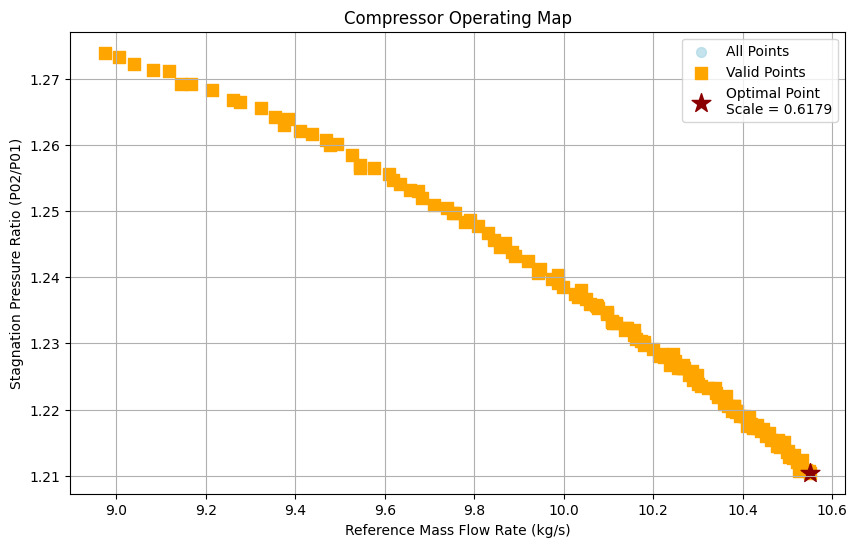
\includegraphics[width=0.8\textwidth]{Figure_1.jpg}
		\caption{\textbf{Compressor Operating Map}}
		\label{fig:compressor_map}
	\end{figure}
	
	The optimal operating point corresponds to the highest achievable scale while satisfying design constraints.
	
	\section*{RESULTS AND DISCUSSION}
	The analysis yielded these key outcomes:
	\begin{itemize}
		\item \textbf{Maximum Achievable Scale:} 0.6179(61.79\% of prototype size)
		\item \textbf{Optimal Operating Parameters:}
		\begin{itemize}
			\item Reference mass flow rate: $ 10.5503 \ \mathrm{kg/s}$
			\item Pressure ratio: 1.2105
			\item Corresponding $p_{01}$: $204.6995 \ \mathrm{kPa}$
		\end{itemize}
		
	\end{itemize}
	
	% Future Work
\section*{Future Work}
The current research facility can be used for experimental analysis for various prototypes with changes to the diffuser and the test section. Three experimental research studies that respect the structural constraints (250 kPa maximum pressure, closed-loop operation) are proposed:

\begin{itemize}
	\item \textbf{Experimental Validation of AI-Optimized Compressor Blades:}
	\begin{itemize}
		\item Validaton of compressor blades or diffusers designed using artificial intelligence and machine learning optimization techniques can be carried out without significant changes.
		\item Testing these advanced geometries under controlled laboratory conditions enables direct assessment of improvements in aerodynamic performance, efficiency, and surge margin.
		\item This research is of significant interest to companies such as \textbf{Siemens Energy, GE Vernova}, and \textbf{Rolls-Royce}, and others who are actively pursuing digital design and rapid prototyping strategies.
	\end{itemize}
	
	\item \textbf{Evaluation of Advanced Turbomachinery Control Systems:}
	\begin{itemize}
		\item Comprehensive testing of new digital controllers, sensors, and actuators intended for compressor surge prevention and efficiency optimization can be carried out in the laboratory.
		\item Exhaustive testing of these control systems in a realistic environment allows for  improvement in algorithms and hardware, ensuring robust performance before field deployment.
		\item This study is particularly relevant for \textbf{ABB, Siemens Energy}, and \textbf{Rockwell Automation}, and others operating in the sphere of retrofitting advanced turbomachinery control solutions.
	\end{itemize}
	
	\item \textbf{Assessment of Oil-Free Bearings and High-Performance Coatings:}
	\begin{itemize}
		\item Testing these technologies under representative pressure and speed conditions allows for the evaluation of bearing life, frictional characteristics, and thermal performance.
		\item This will further the rapid adoption of maintenance-free and high-reliability solutions in both aerospace and industrial sectors, and is of direct benefit to companies such as \textbf{Williams International, Mohawk Innovative Technologies,} and \textbf{GE Vernova}.
	\end{itemize}
\end{itemize}
	% Supplement
	\section*{SUPPLEMENT}
	The following files are included with this report:
	\begin{enumerate}
		\item Python code file: `sol.py`
		\item LaTeX files: Provided as a .zip file for compilation.
	\end{enumerate}
	
	---
\end{document}
	